\begin{minipage}{.3\textwidth}
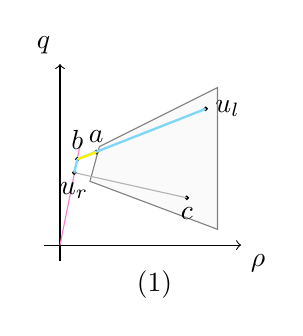
\begin{tikzpicture}
% coordinates
    \filldraw[fill=black!2, draw=black!50] plot [tension = 1] coordinates { (0.5,1.25) (2,2) (2,0.2) (0.38, 0.81) (0.5,1.25)};
    \draw[->] (0,-0.2) -- (0,2.3) node[anchor=south east] {$q$};
    \draw[->] (-0.2,0) -- (2.3,0) node[anchor=north west] {$\rho$};

    \draw[magenta!50] (0,0) -- (0.25,1.25) ;
    
    \filldraw[black] (0.46,1.18) circle (0.6pt) node[anchor = south ]{$a$} ;
    \filldraw[black] (0.22,1.09) circle (0.6pt) node[anchor = south ]{$b$};
    
    \filldraw[black] (1.85,1.73) circle (0.6pt) node[anchor = west]{$u_l$} ;
    \filldraw[black] (0.18,0.92) circle (0.6pt) node[anchor = north ]{$u_r$} ;
    \filldraw[black] (1.61,0.6) circle (0.6pt) node[anchor = north]{$c$};
    
     \draw[-][line width=0.3mm,cyan!50] (0.22,1.09) -- (1.85,1.73) ;
     \draw[-][black!30] (0.18,0.92)  -- (1.61,0.6) ;
     \draw[-][line width=0.3mm,yellow] (0.46,1.18) -- (0.22,1.09) ;
     \draw[-][line width=0.3mm,cyan!50] (0.22,1.09) -- (0.18,0.92)  ;
  
     \node at (1.2,-0.5) {$(1)$};
     % rarefactions and shocks
    %\draw[lime] (1.05, 1.33) -- (2, 1.6) ;
    %\draw[<-][cyan!50] (0.42, 1.19) -- (1, 1.33) ;
    
    %\draw[->][lime] (1.48,0.4)  -- (2, 0.2) ;
    %\draw[-][cyan!50] (0.48,1.2) -- (1.8,1.55)   ;
    %\draw[yellow] (0.135,1.05) -- (0.45,1.11);
    
    % contacts
    \draw[ black!30, domain=1.3:1.86]  plot[id=x] function{(x/1.61)*(2-1.61)/(2-x)*0.6};
    %\draw[ orange!50, domain=0:1.28]  plot[id=x] function{(x/1.16)*(2-1.16)/(2-x)*1.63};
     
\end{tikzpicture}
\end{minipage}
\begin{minipage}{.3\textwidth}
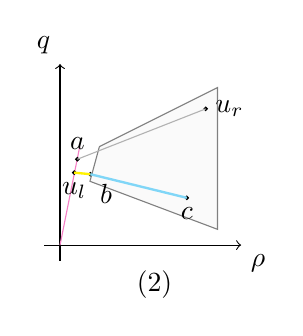
\begin{tikzpicture}
% coordinates
    \filldraw[fill=black!2, draw=black!50] plot [tension = 1] coordinates { (0.5,1.25) (2,2) (2,0.2) (0.38, 0.81) (0.5,1.25)};
    \draw[->] (0,-0.2) -- (0,2.3) node[anchor=south east] {$q$};
    \draw[->] (-0.2,0) -- (2.3,0) node[anchor=north west] {$\rho$};

    \draw[magenta!50] (0,0) -- (0.25,1.25) ;
    
    \filldraw[black] (0.385,0.9) circle (0.6pt) node[anchor = north west ]{$b$} ;
    \filldraw[black] (0.22,1.09) circle (0.6pt) node[anchor = south ]{$a$};
    \filldraw[black] (1.85,1.73) circle (0.6pt) node[anchor = west]{$u_r$} ;
    \filldraw[black] (0.18,0.92) circle (0.6pt) node[anchor = north ]{$u_l$} ;
    \filldraw[black] (1.61,0.6) circle (0.6pt) node[anchor = north]{$c$};
    
     \draw[-][black!30] (0.22,1.09) -- (1.85,1.73) ;
     \draw[-][line width=0.3mm, yellow] (0.18,0.92)  -- (0.385,0.9) ;
     \draw[-][line width=0.3mm,cyan!50] (0.385,0.9)  -- (1.61,0.6) ;
  
     \node at (1.2,-0.5) {$(2)$};
     % rarefactions and shocks
    %\draw[lime] (1.05, 1.33) -- (2, 1.6) ;
    %\draw[<-][cyan!50] (0.42, 1.19) -- (1, 1.33) ;
    
    %\draw[->][lime] (1.48,0.4)  -- (2, 0.2) ;
    %\draw[-][cyan!50] (0.48,1.2) -- (1.8,1.55)   ;
    %\draw[yellow] (0.135,1.05) -- (0.45,1.11);
    
    % contacts
    \draw[line width=0.3mm, orange!90, domain=1.3:1.86]  plot[id=x] function{(x/1.61)*(2-1.61)/(2-x)*0.6};
    %\draw[ orange!50, domain=0:1.28]  plot[id=x] function{(x/1.16)*(2-1.16)/(2-x)*1.63};
     
\end{tikzpicture}
\end{minipage}
\begin{minipage}{.3\textwidth}
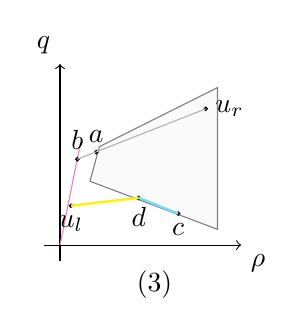
\begin{tikzpicture}
% coordinates
    \filldraw[fill=black!2, draw=black!50] plot [tension = 1] coordinates { (0.5,1.25) (2,2) (2,0.2) (0.38, 0.81) (0.5,1.25)};
    \draw[->] (0,-0.2) -- (0,2.3) node[anchor=south east] {$q$};
    \draw[->] (-0.2,0) -- (2.3,0) node[anchor=north west] {$\rho$};

    \draw[magenta!50] (0,0) -- (0.25,1.25) ;
    
    \filldraw[black] (0.46,1.18) circle (0.6pt) node[anchor = south ]{$a$} ;
    \filldraw[black] (0.22,1.09) circle (0.6pt) node[anchor = south ]{$b$};
    \filldraw[black] (1.85,1.73) circle (0.6pt) node[anchor = west]{$u_r$} ;
    \filldraw[black] (0.14,0.5) circle (0.6pt) node[anchor = north ]{$u_l$} ;
    \filldraw[black] (1.5,0.4) circle (0.6pt) node[anchor = north]{$c$};
    \filldraw[black] (1,0.6) circle (0.6pt) node[anchor = north]{$d$};
    
     \draw[-][black!30] (0.22,1.09) -- (1.85,1.73) ;
     \draw[-][line width=0.3mm, yellow] (0.14,0.5)  -- (1,0.6) ;
     \draw[-][line width=0.3mm, cyan!50](1,0.6)  -- (1.5,0.4) ;
  
     \node at (1.2,-0.5) {$(3)$};
     % rarefactions and shocks
    %\draw[lime] (1.05, 1.33) -- (2, 1.6) ;
    %\draw[<-][cyan!50] (0.42, 1.19) -- (1, 1.33) ;
    
    %\draw[->][lime] (1.48,0.4)  -- (2, 0.2) ;
    %\draw[-][cyan!50] (0.48,1.2) -- (1.8,1.55)   ;
    %\draw[yellow] (0.135,1.05) -- (0.45,1.11);
    
    % contacts
    \draw[line width=0.3mm, orange!90, domain=1.3:1.86]  plot[id=x] function{(x/1.61)*(2-1.61)/(2-x)*0.6};
    %\draw[ orange!50, domain=0:1.28]  plot[id=x] function{(x/1.16)*(2-1.16)/(2-x)*1.63};
     
\end{tikzpicture}
\end{minipage}
\begin{minipage}{.3\textwidth}
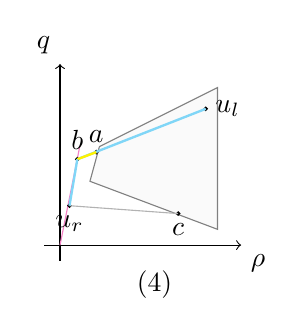
\begin{tikzpicture}
% coordinates
    \filldraw[fill=black!2, draw=black!50] plot [tension = 1] coordinates { (0.5,1.25) (2,2) (2,0.2) (0.38, 0.81) (0.5,1.25)};
    \draw[->] (0,-0.2) -- (0,2.3) node[anchor=south east] {$q$};
    \draw[->] (-0.2,0) -- (2.3,0) node[anchor=north west] {$\rho$};

    \draw[magenta!50] (0,0) -- (0.25,1.25) ;
    
    \filldraw[black] (0.46,1.18) circle (0.6pt) node[anchor = south ]{$a$} ;
    \filldraw[black] (0.22,1.09) circle (0.6pt) node[anchor = south ]{$b$};
    \filldraw[black] (1.85,1.73) circle (0.6pt) node[anchor = west]{$u_l$} ;
    \filldraw[black] (0.12,0.5) circle (0.6pt) node[anchor = north ]{$u_r$} ;
    \filldraw[black] (1.5,0.4) circle (0.6pt) node[anchor = north]{$c$};

    
     \draw[-][black!30] (0.22,1.09) -- (1.85,1.73) ;
     \draw[-][black!30] (0.12,0.5)  -- (1.5,0.4) ;
      \draw[-][line width=0.3mm,cyan!50] (0.22,1.09) -- (1.85,1.73) ;
     \draw[-][line width=0.3mm,yellow] (0.46,1.18) -- (0.22,1.09) ;
     \draw[-][line width=0.3mm,cyan!50] (0.22,1.09) -- (0.12,0.5) ;
  
     \node at (1.2,-0.5) {$(4)$};
     % rarefactions and shocks
    %\draw[lime] (1.05, 1.33) -- (2, 1.6) ;
    %\draw[<-][cyan!50] (0.42, 1.19) -- (1, 1.33) ;
    
    %\draw[->][lime] (1.48,0.4)  -- (2, 0.2) ;
    %\draw[-][cyan!50] (0.48,1.2) -- (1.8,1.55)   ;
    %\draw[yellow] (0.135,1.05) -- (0.45,1.11);
    
    % contacts
    \draw[ black!30, domain=1.3:1.86]  plot[id=x] function{(x/1.61)*(2-1.61)/(2-x)*0.6};
    %\draw[ orange!50, domain=0:1.28]  plot[id=x] function{(x/1.16)*(2-1.16)/(2-x)*1.63};
     
\end{tikzpicture}
\end{minipage}
\begin{minipage}{.3\textwidth}
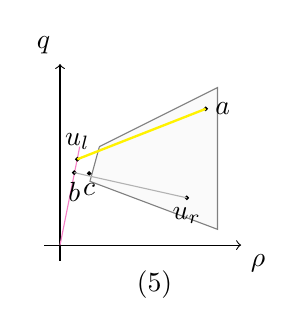
\begin{tikzpicture}
% coordinates
    \filldraw[fill=black!2, draw=black!50] plot [tension = 1] coordinates { (0.5,1.25) (2,2) (2,0.2) (0.38, 0.81) (0.5,1.25)};
    \draw[->] (0,-0.2) -- (0,2.3) node[anchor=south east] {$q$};
    \draw[->] (-0.2,0) -- (2.3,0) node[anchor=north west] {$\rho$};

    \draw[magenta!50] (0,0) -- (0.25,1.25) ;
    
    
    \filldraw[black] (0.22,1.09) circle (0.6pt) node[anchor = south ]{$u_l$};
    \filldraw[black] (1.85,1.73) circle (0.6pt) node[anchor = west]{$a$} ;
    \filldraw[black] (0.18,0.92) circle (0.6pt) node[anchor = north ]{$b$} ;
    \filldraw[black] (0.37,0.91) circle (0.6pt) node[anchor = north ]{$c$} ;
    \filldraw[black] (1.61,0.6) circle (0.6pt) node[anchor = north]{$u_r$};
    
     \draw[-][line width=0.3mm, yellow] (0.22,1.09) -- (1.85,1.73) ;
     \draw[-][black!30] (0.18,0.92)  -- (1.61,0.6) ;
  
     \node at (1.2,-0.5) {$(5)$};
     % rarefactions and shocks
    %\draw[lime] (1.05, 1.33) -- (2, 1.6) ;
    %\draw[<-][cyan!50] (0.42, 1.19) -- (1, 1.33) ;
    
    %\draw[->][lime] (1.48,0.4)  -- (2, 0.2) ;
    %\draw[-][cyan!50] (0.48,1.2) -- (1.8,1.55)   ;
    %\draw[yellow] (0.135,1.05) -- (0.45,1.11);
    
    % contacts
    \draw[ line width=0.3mm, orange!90, domain=1.3:1.86]  plot[id=x] function{(x/1.61)*(2-1.61)/(2-x)*0.6};
    %\draw[ orange!50, domain=0:1.28]  plot[id=x] function{(x/1.16)*(2-1.16)/(2-x)*1.63};
     
\end{tikzpicture}
\end{minipage}
\begin{minipage}{.3\textwidth}
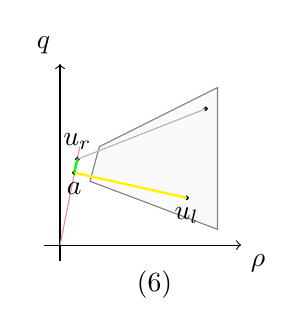
\begin{tikzpicture}
% coordinates
    \filldraw[fill=black!2, draw=black!50] plot [tension = 1] coordinates { (0.5,1.25) (2,2) (2,0.2) (0.38, 0.81) (0.5,1.25)};
    \draw[->] (0,-0.2) -- (0,2.3) node[anchor=south east] {$q$};
    \draw[->] (-0.2,0) -- (2.3,0) node[anchor=north west] {$\rho$};

    \draw[magenta!50] (0,0) -- (0.25,1.25) ;
    
    
    \filldraw[black] (0.22,1.09) circle (0.6pt) node[anchor = south ]{$u_r$};
    \filldraw[black] (1.85,1.73) circle (0.6pt) ;
    \filldraw[black] (0.18,0.92) circle (0.6pt) node[anchor = north ]{$a$} ;
    \filldraw[black] (1.61,0.6) circle (0.6pt) node[anchor = north]{$u_l$};
    
     \draw[-][black!30] (0.22,1.09) -- (1.85,1.73) ;
     \draw[-][line width=0.3mm, yellow] (0.18,0.92)  -- (1.61,0.6) ;
     \draw[-][line width=0.3mm, green] (0.18,0.92) -- (0.22,1.09); 
  
     \node at (1.2,-0.5) {$(6)$};
     % rarefactions and shocks
    %\draw[lime] (1.05, 1.33) -- (2, 1.6) ;
    %\draw[<-][cyan!50] (0.42, 1.19) -- (1, 1.33) ;
    
    %\draw[->][lime] (1.48,0.4)  -- (2, 0.2) ;
    %\draw[-][cyan!50] (0.48,1.2) -- (1.8,1.55)   ;
    %\draw[yellow] (0.135,1.05) -- (0.45,1.11);
    
    % contacts
    \draw[ black!30, domain=1.3:1.86]  plot[id=x] function{(x/1.61)*(2-1.61)/(2-x)*0.6};
    %\draw[ orange!50, domain=0:1.28]  plot[id=x] function{(x/1.16)*(2-1.16)/(2-x)*1.63};
     
\end{tikzpicture}
\end{minipage}